\documentclass{article}
\usepackage[utf8]{inputenc}
\usepackage[margin = 0.8in]{geometry}
\usepackage{graphicx}
\usepackage{amsmath, amssymb}
\usepackage{caption}
\usepackage{subcaption}
\usepackage{multirow}
\usepackage{multicol}
\usepackage{booktabs}
\usepackage{bm}
\setlength{\columnsep}{.75cm}
\usepackage{float}
\usepackage{graphicx}
\usepackage{stfloats}
\usepackage{hyperref}
\graphicspath{ {./images/} }
\setcounter{MaxMatrixCols}{15}

%\usepackage[parfill]{parskip}. %to not indent paragraph
\renewcommand\refname{References}
\restylefloat{table}


\title{LQR Control of a Nonlinear Quadrotor System}
\author{Keith Chester, Bob DeMont, Sean Hart}
\date{November 9th, 2021}

\begin{document}

\maketitle

\begin{multicols}{2}
\section*{Abstract}
The purpose of the project is to simulate the control and stable flight of an unmanned four rotor flying vehicle known as a quadrotor.  The problem is set into three goals: simulation and control of the quadrotor hover in a stable configuration, intercept a unknown drone's flight path, and return with the captured target quadrotor with randomized disturbance forces while maintaining stable flight.

\section*{Introduction}
The mission is the defense of a designated airspace.  Our quadrotor is assigned to guard a limited airspace, launch if an unidentified UAV enters that airspace, capture the target, and return to base.  If the target leaves the airspace before being captured, our quadrotor should return to base.  When captured, the target should be assumed to generate external forces and moments on our UAV.

\section*{Methodology}
\textbf{General Approach}.  We'll begin by generating the state space variables and defining the equations that define the state space.  We'll prove controllability of the system and choose a controller methodology.  Using the controller, we will simulate hovering as well as moving to a location and hovering. Finally we'll introduce external forces and moments that would be experienced by simulating a target capture in the problem statement. In order to simulate the quadrotor and its flight dynamics, the design will be coded into MATLAB, using an ODE solver to compute the state variables, with full state variables, A and B matrices, K gain matrix, $K_{capture}$ gain matrix (incorporating $n$ and $r$ forces and torques from the target), as well as characteristics for graphing.\\

\noindent \textbf{Frames and Constants}.  Coordinate frames are identified for the reference/inertial frame $E={[e_1, e_2, e_3]}$ at the center bottom of the airspace and the body frame $C={[c_1, c_2, c_3]}$. All rotors are equidistant from the center of mass and in the same x-y plane as the body's center of mass. The external forces and moments on the system are represented by $\boldsymbol{r}$ and $\boldsymbol{n}$, where $\boldsymbol{r} = r_1 c_1 + r_2 c_2 + r_3 c_3$ and $\boldsymbol{n} = n_1 c_1 + n_2 c_2 + n_3 c_3$ are directly applied to the center of mass. We are assuming that the torque of the rotor is proportionally related to the input thrust via the constant $\sigma>0$, for $\tau_i = \sigma u_i$. We will be utilizing $\boldsymbol{I}$ as our diagonal inertial matrix where diagonal elements  $I_x, I_y $, and $I_z$ represent the mass moments of inertia about $c_1, c_2 $, and $c_3$ respectively. For the purpose of our analysis we will assume simplified aerodynamic effects and ignore  drag, ground effects, translational lift, blade flapping, feathering and lagging, and other aerodynamic complexities. The parameters for our state are described in Table 1 of reference \cite{FaalP}\\.

\noindent \textbf{State Variable}.  Development of the quadrotor state equations are found in \cite{FaalD}.  We'll establish the state variable, $\mathbf{z}$, to represent the quadrotor's xyz center-of-mass position in the earth frame $\mathbf{x}=\begin{bmatrix}x_1 & x_2 & x_3\end{bmatrix}^T$; the roll, pitch, yaw angles in the earth frame, $\bm{\alpha} =\begin{bmatrix}\phi & \theta & \psi\end{bmatrix}^T$; the xyz linear velocities in the earth frame, $\mathbf{v}=\begin{bmatrix}v_1 & v_2 & v_3\end{bmatrix}^T$; and the angular accelerations $\bm{\omega}=\begin{bmatrix}\omega_1 & \omega_2 & \omega_3\end{bmatrix}^T$ in the earth roll pitch yaw directions. Thus our state variable is $\mathbf{z}=\begin{bmatrix}\mathbf{x} &\bm{\alpha}&\mathbf{v}&\bm{\omega}\end{bmatrix}^T$. We define $\boldsymbol{\dot{z}}$ as $\begin{bmatrix} \mathbf{\dot{x}} &\bm{\dot{\alpha}}&\mathbf{\dot{v}}&\bm{\dot{\omega}} \end{bmatrix}^T$, with:

\begin{equation}
    \mathbf{\dot{x}} =\mathbf{v}
\end{equation}
\begin{equation}
    \bm{\dot{\alpha}} =\mathbf{T}^{-1}\bm{\omega}
\end{equation}
\begin{align}
    \mathbf{\dot{v}} &=-ge_3+\frac{1}{m}\mathbf{R_{C/E}}(u_1+u_2+u_3+u_4)c_3 \nonumber\\ &+\frac{1}{m}\mathbf{R_{C/E}}r
\end{align}
\begin{align}
    \bm{\dot{\omega}} &=I^{-1}((u_2-u_4)lc_1+(u_3-u_1)lc_2 \nonumber\\ &+(u_1-u_2+u_3-u_4)\sigma c_3+n-\omega \times I \omega)
\end{align}

\noindent ...where $\mathbf{R_{C/E}}$ is defined in the problem statement as the Euler rotation matrix from quadrotor frame $C$ to earth frame $E$ and $\mathbf{T}^{-1}$, also defined in the problem statement, relates the angular rate of change of the Euler angles based on the angular velocity of the quadrotor.

Our system is nonlinear because it is under-actuated; four actuators for six degrees of freedom. We can utilize linearization to simplify this model and approximate its behaviour for easier control. To do this,  approximate our system as $\boldsymbol{\dot{z}}=\boldsymbol{A}\boldsymbol{x}+\boldsymbol{B}\boldsymbol{u}$. We derive the $\boldsymbol{A}$ matrix as the Jacobian of our $\boldsymbol{\dot{z}}$ by $\boldsymbol{z}$, and our $\boldsymbol{B}$ as the Jacobian of our $\boldsymbol{\dot{z}}$ by $\boldsymbol{u}$. 

For our approximation we model the quadrotor in a stable hovering position, where a given state is $\boldsymbol{z}=\begin{bmatrix} 
x & y & z & \boldsymbol{0}\end{bmatrix}^T$; no velocities, accelerations, and its orientation level. We assume a base output of $
\frac{mg}{4}$, or each motor outputing the necessary force of a hover. We assign these values to our derived $\boldsymbol{A}$ and 
$\boldsymbol{B}$ matricies.

We then confirm that our system is controllable with these matricies. We create a controllability matrix $\boldsymbol{C}$, 
which we define as $\boldsymbol{C} = \begin{bmatrix} A^0B & A^1B & A^2B & \dots & A^{n-3}B & A^{n-2}B & A^{n-1}B\end{bmatrix}$ 
where $n$ is the size of our input, $12$. We must ensure that the combinations of our state and input matrices are linearly 
independent to the degree that we have an independent column for each state. To do so, we check rank of the controllability matrix $
\boldsymbol{C}$ to assure that we have rank equal to the number of states in our z vector. As expected, the rank of our derived 
controllabiltiy matrix is indeed $12$.

We can utilize these to derive our $\boldsymbol{K}$ matrix to create a Linear-Quadratic Regulator (LQR) controller.

\section*{LQR Controller}
We selected the Linear-Quadratic Regulator (LQR) approach as an optimal control technique for generating the gain matrix, $
\boldsymbol{K}$.  LQR operates on our linearized system, utilizing both $\boldsymbol{A}$ and $\boldsymbol{B}$ matricies (states 
and inputs, respectively). LQR also utilizes two additional matrices- $\boldsymbol{Q}$ and $\boldsymbol{R}$, which correspond to $
\boldsymbol{A}$ and $\boldsymbol{B}$, respectively. $\boldsymbol{Q}$'s and $\boldsymbol{R}$'s purpose are to impose a weighted 
cost such that there will be trade off between particular elements of the state and inputs in the optimization. Since we are not asked 
to weigh the cost of using our actuators (as if we were conserving fuel), we have initially left both the  4x4 $\boldsymbol{R}$ matrix 
and 12x12 $\boldsymbol{Q}$ matrices as identity matrices, but found through experimentation that our 
desired performance required adjustments( to be discussed later in this paper). There is an additional matrix, $\boldsymbol{N}$, 
which acts as a penalty to the interactions between state variables and inputs.  We simplify by omitting this matrix.

LQR acts on the linearized system of the form $\dot{x} = Ax + Bu$ and calculates a cost function based on optimization.  This 
integrates the costs of both $\boldsymbol{Q}$ and $\boldsymbol{R}$ for comparison:
\begin{equation}
J =x_0^TF(0)x(t_0) +  \int_{t_0}^{t_f} x^TQx+u^TRu +2x^TNu\,dt 
\end{equation}

The control input u that minimizes this cost function is $u= -Kx$ with the K value is given by
\begin{equation}
K = R^{-1}(B^TP(t) + N^T)
\end{equation}
\noindent
Where P is created by solving Ricatti's continuous time differential equation:
\begin{align}
A^TP(t) + P(t)A - (P(t)B + N)R^{-1}(B^TP(t) + N^T) \nonumber\\+ Q = \dot{P}(t)
\end{align}
\noindent
and $P(t)$ is bounded by $P(0) = F(0)$. This process is repeated as we experimented with adjusting the weights within the $
\boldsymbol{Q}$ matrix.

Once we have our calculated $\boldsymbol{K}$, we define $z_d$ as the desired state of our quadrotor. If we are hovering  
at a given point in space, it will be $z_d=\begin{bmatrix} x_{1_d} & x_{2_d} & x_{3_d} & \boldsymbol{0} 
\end{bmatrix}^T$. When we are chasing a given target through protected airspace, we will set the desired state to 
$z_d(t)=\begin{bmatrix} x_t(t) & \boldsymbol{0} \end{bmatrix}^T$ where $x_t(t)$ is the given xyz position of the target at a given 
time $t$. We then calculate the error $e(t)$ as the difference between our desired state, or $z_d - z$. We utilize the error to 
determine the resulting inputs to our system, but we also must take note that since we assumed a linearized system around 
hovering, we must add an additional force of $\frac{mg}{4}$ to each of our input forces. Thus $\boldsymbol{u}= \boldsymbol{K}e(t) + 
\begin{bmatrix}\frac{mg}{4} & \frac{mg}{4} & \frac{mg}{4} & \frac{mg}{4}\end{bmatrix}$. 
Once we have calculated our $\boldsymbol{u}$, we limit the resulting outputs to to $u\  \epsilon\  (0, 3)$ as that is the maximum and minimum thrust our motors can generate. We then utilize the MATLAB ode45 solver, with our previously derived $\boldsymbol{\dot{z}}$ and calculated $\boldsymbol{u}$. At each stage we determine what state of behavior we desire from our quadrotor - hover, move, or intercept - and from this determine the $z_d$. We then solve for our state variable $\boldsymbol{z}$ at each time increment.

\section*{Simulation}
\noindent
The foundation of simulating the controller are the solutions of the system of differential equations of our original system with the added 
gain from our LQR controller.  We have wrapped the changes in the environment into a separate function to serve as the ODE 
function in order to incorporate time-related changes to the target path as well as $n$ and $r$ torques and forces after capture.\\
\textbf{Quadrotor Hovering.}. To demonstrate successful control of our quadrotor, we establish an initial state of $z=[\mathbf{0}]^T$ and 
a desired state $z_d=[5,5,5,\boldsymbol{0}]^T $ to demonstrate move and hover.  Feeding these into our ode45 solver, we obtain 
smooth movement and hovering at the given $z_d$.  (Noting initial and final states as well as the trajectory plotted) in Figure 1a.\\
\textbf{Quadrotor Return to Base}. A mission objective was to return to base if the target exits the envelope before capture.  
Figure 1b. demonstrates this performance. In this scenario the interceptor leaves the base to pursue the target, but the target exits 
the airspace envelope before the interceptor gets close enough to capture.\\
\textbf{Quadrotor Interception of Target}. For modeling we will input a continuous function for the target so that we can include it in a single differentiation.  In earlier iterations, we coded random, continuous movements into the target which were only 
revealed to our quadrotor each second in a loop.  We resolved the ODE for new $z_d$ in that loop and were readily able to converge, so we believe the known "unknown" target trajectory to be an allowable simplification for solved time. For interception, it is assumed that the target is intercepted if we get within a distance of 0.3 meters of it. Our simulation demonstrates successful interception of the target after tuning the Q matrix to mitigate errors in the z direction (to enable smoother up and down 
movement) and penalize x-y errors.  \\
\textbf{Capture Drone and Return to Base  with Disturbances}.  For the disturbance 
forces and torques after capture,  in the code of the ODE function we trigger a 
change in $n$ and $r$ and re-evaluate K  to recalculate the control, $u$, term for the 
ODE.  Mission parameters asked to reach an $||n||\leq1$ (moment) and $||r||\leq2$ (force). We began by testing constant moments and forces in each direction before mixing or randomizing since the system must, at a minimum, handle a constant force of the required magnitude before being able to deal with a time-dependent randomized force.
\begin{figure}[H]
\centering
\begin{subfigure}[b]{0.49\columnwidth}
    \centering
    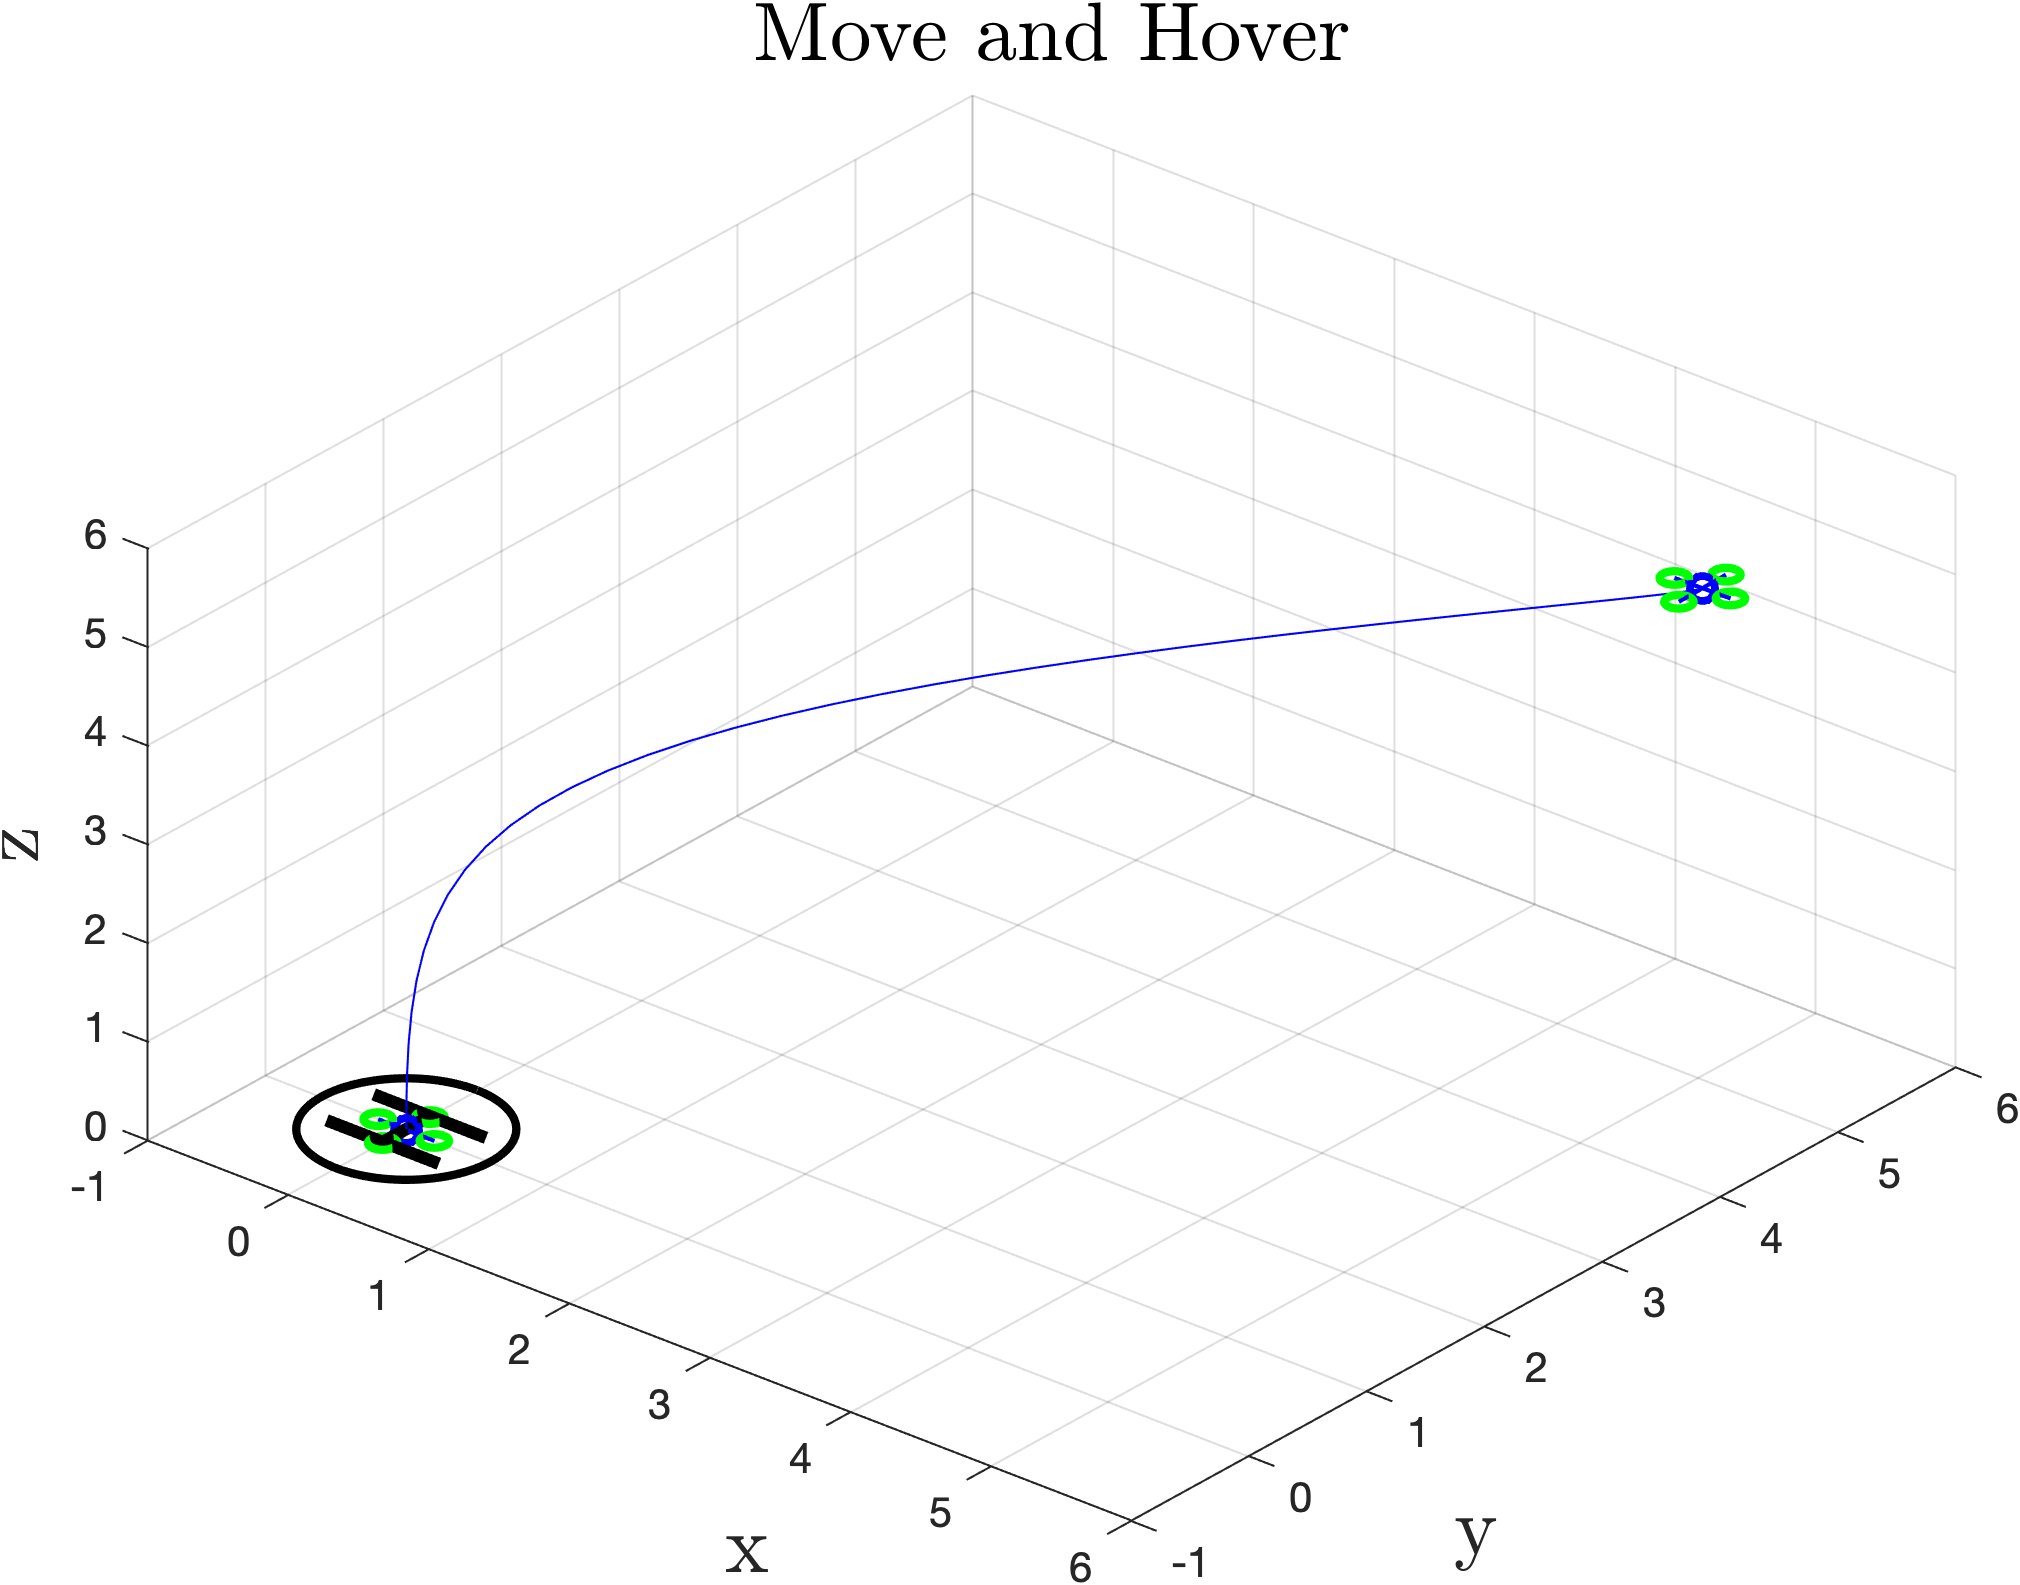
\includegraphics[width = 1\textwidth]{images/MoveAndHover.png}
     \label{fig:MandH}
     \vspace{-5mm}
     \caption{Move and Hover}
\end{subfigure}
\begin{subfigure}[b]{0.49\columnwidth}
    \centering
    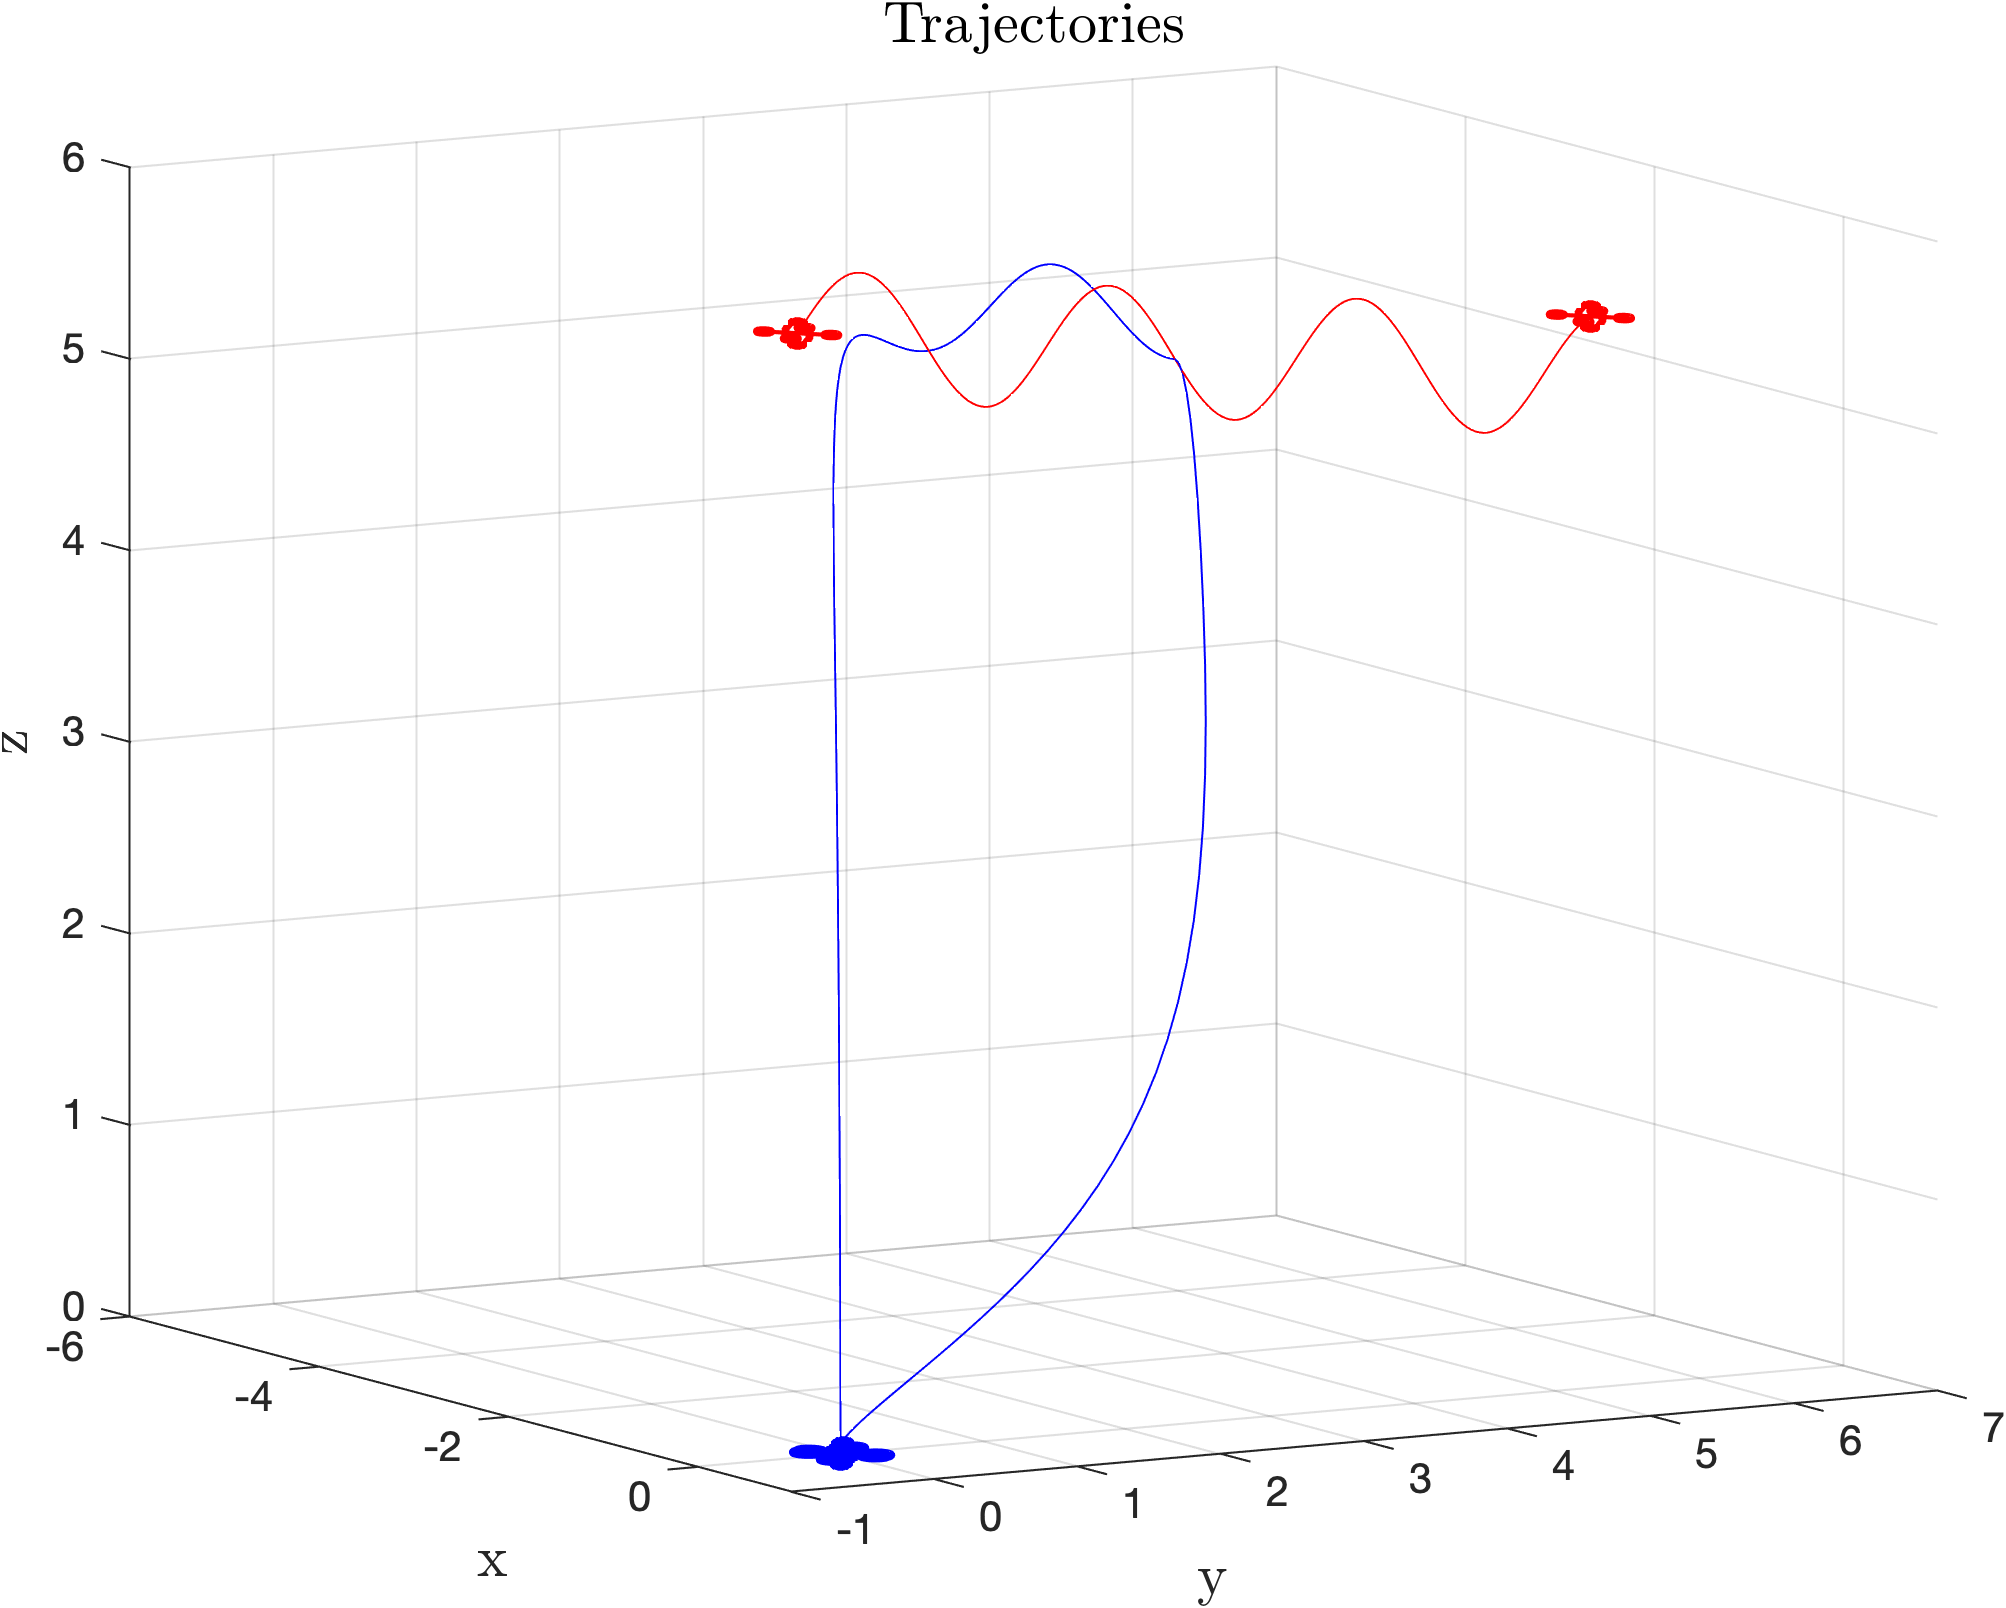
\includegraphics[width = 1\textwidth]{images/ReturnToBase.png}
     \label{fig:Return}
     \vspace{-5mm}
      \caption{Return to Base}
 \end{subfigure}
\begin{subfigure}[b]{0.49\columnwidth}
    \centering
    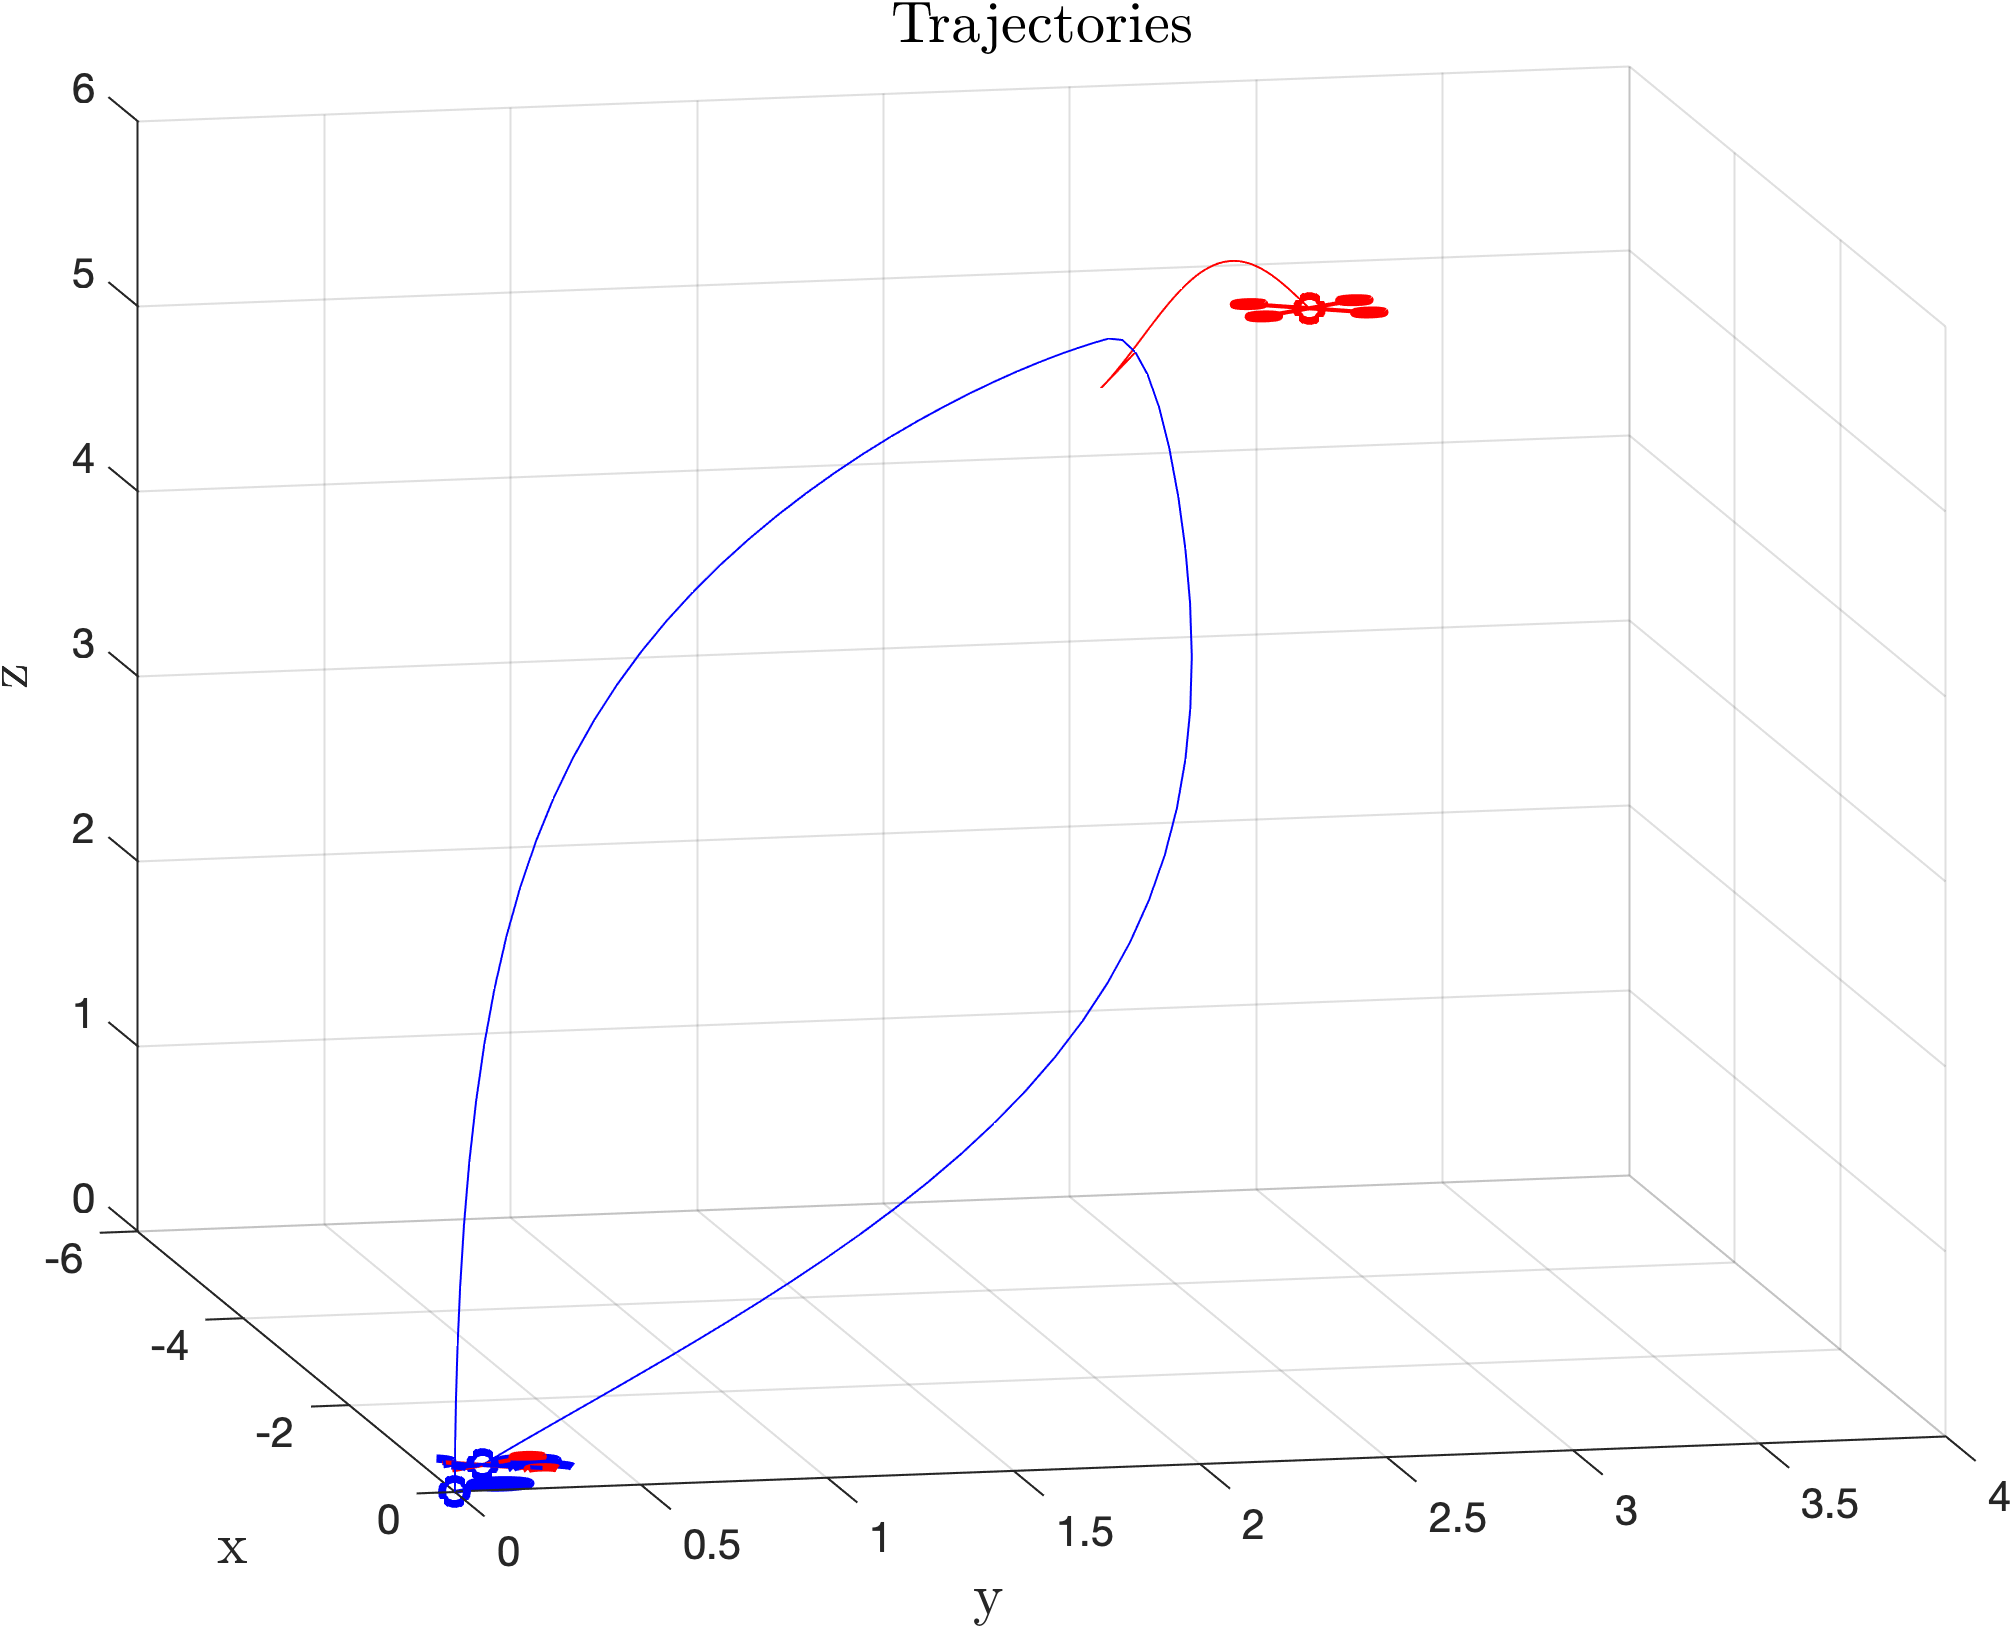
\includegraphics[width = 1\textwidth]{images/Intercept.png}
     \label{fig:Capture}
     \vspace{-5mm}
     \caption{Capture}
 \end{subfigure}
 \begin{subfigure}[b]{0.49\columnwidth}
    \centering
    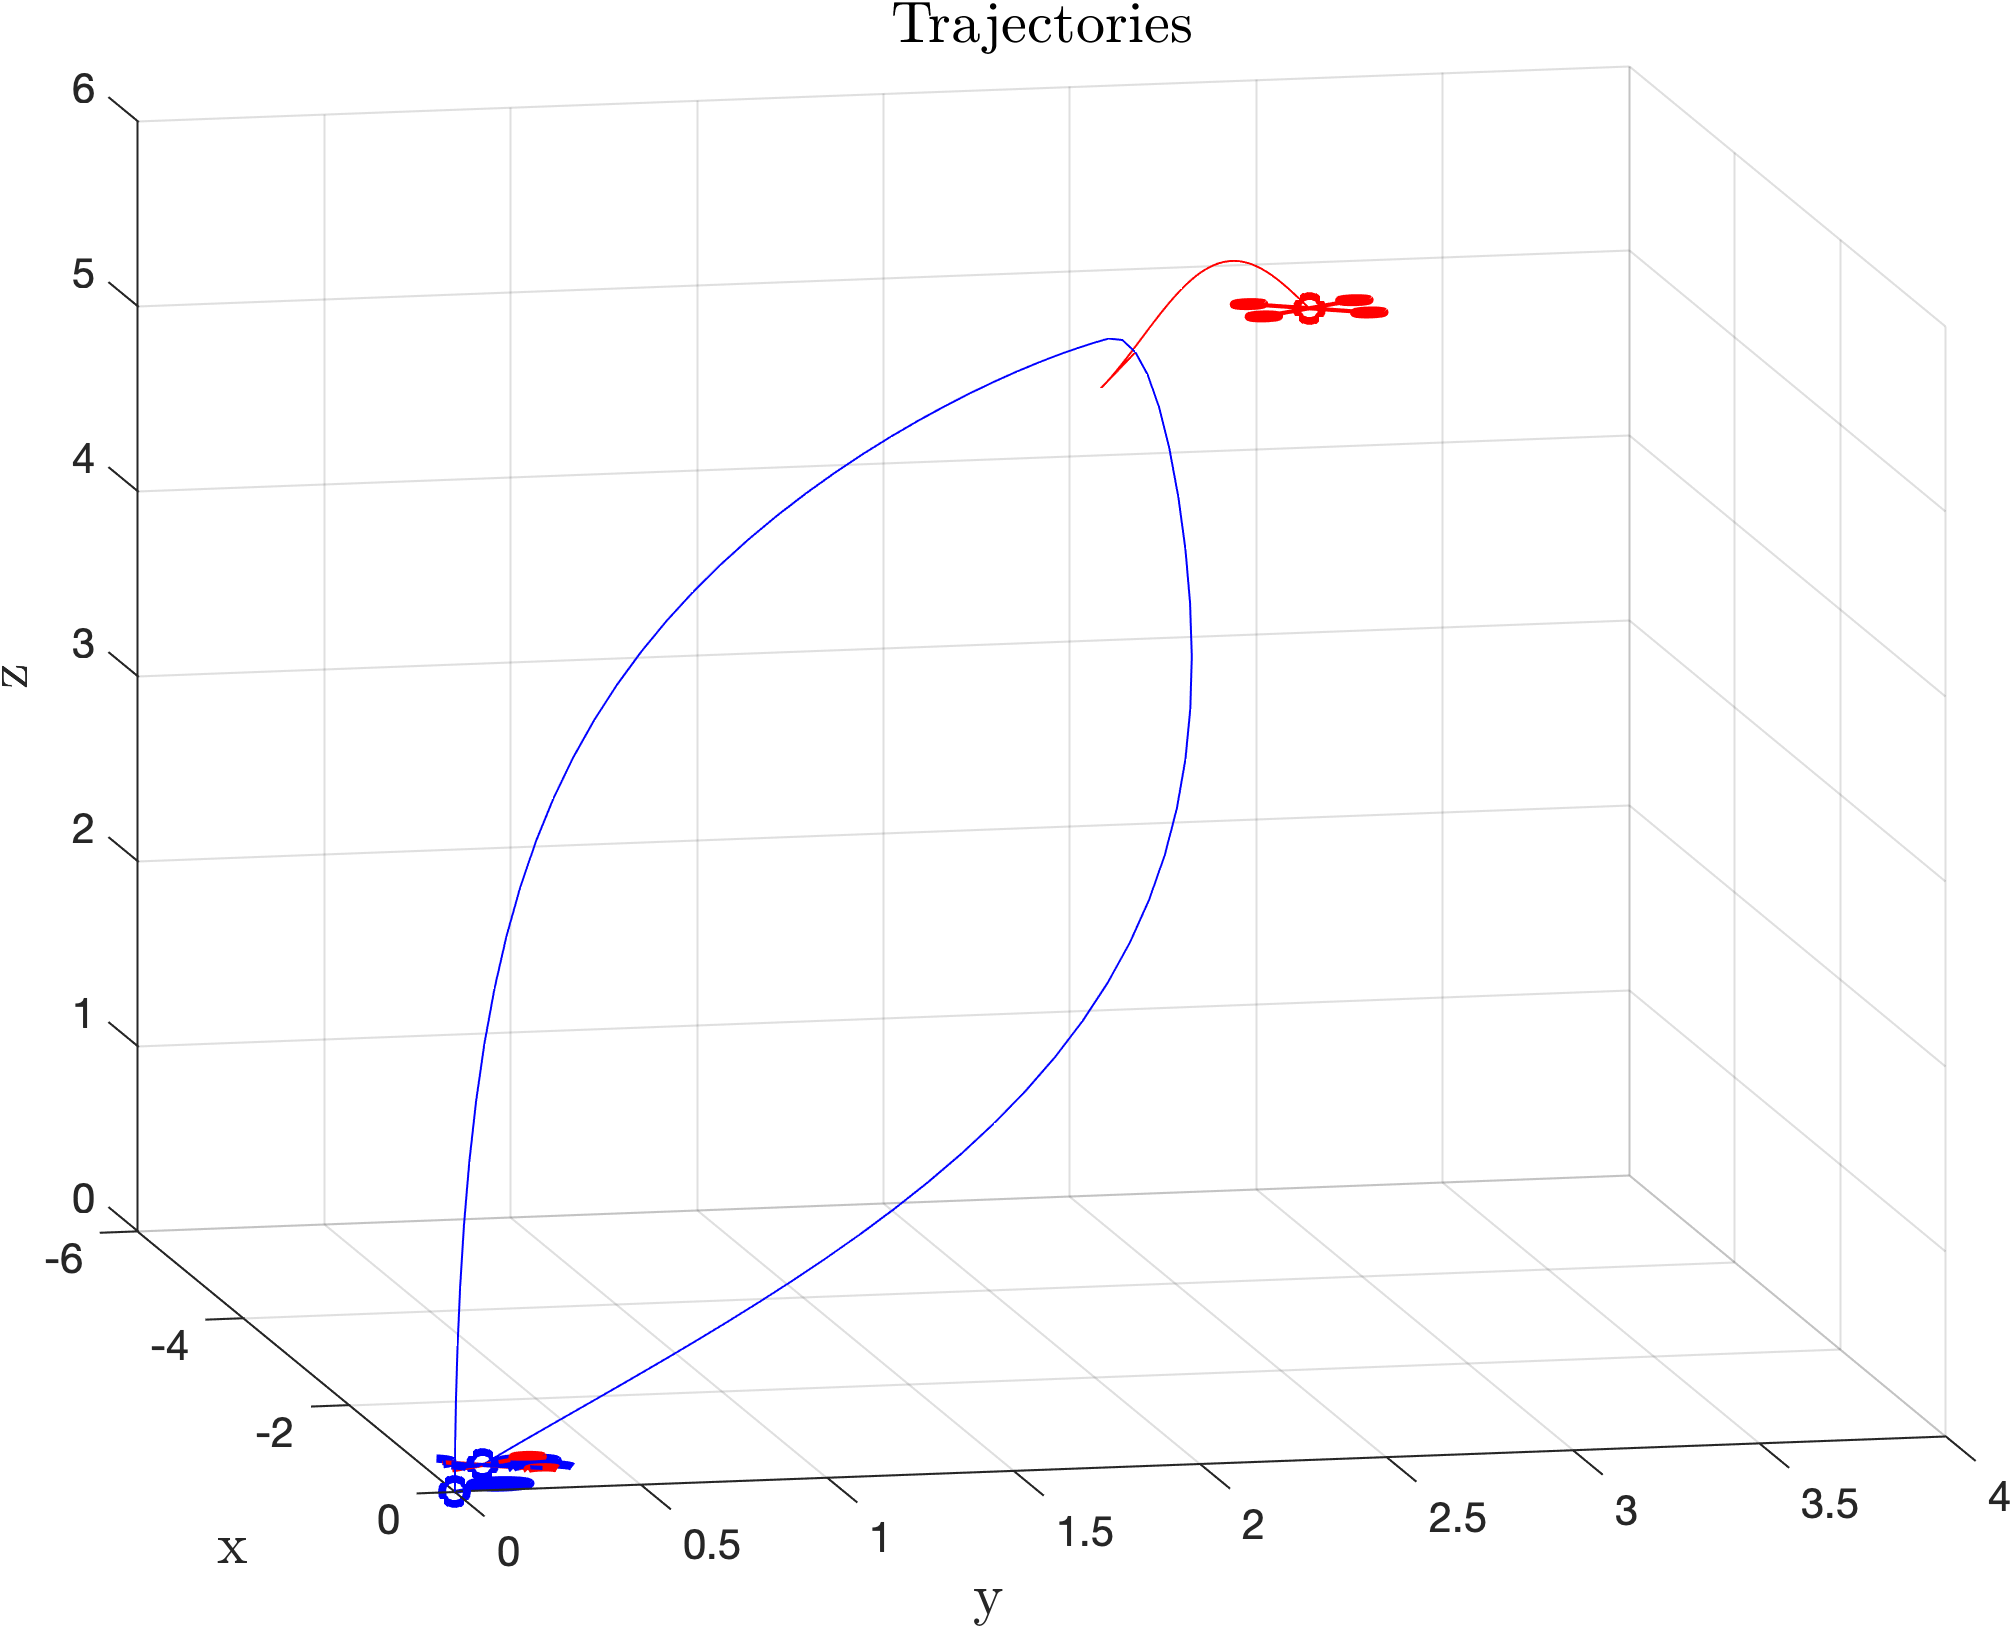
\includegraphics[width = 1\textwidth]{images/Intercept.png}
     \label{fig:CaptureW}
     \vspace{-5mm}
     \caption{Capture Disturbance}
 \end{subfigure}
   \caption{Quadrotor Performance Tests}
\end{figure}

\section*{Results}
As noted above, the LQR controller successfully handled move and hover, return to base, and intercept missions.  We encountered less successful results with strong disturbances after capture.\\
\textbf{Forces}.  To explore, we began simulating constant force in the $c_1$ direction to understand how our $Q_{(4,4)}$ term for roll would be impacted.  At $Q_{(4,4)}=1$ and $n=\begin{bmatrix}1 & 0 & 0\end{bmatrix}$ the system did not converge on an equilibrium and began a catastrophic tumbling beginning with pitch angle. Due to the tumbling we hypothesized that near level flight i.e. preventing roll and pitch from exceeding $\frac{\pi}{4}$, would benefit control especially since the forces are acting in the $c$ frame which causes an outsize effect in $e$.  Compensating for the tumbling by increasing $Q_{(4,4)}$ and $Q_{(5,5)}$ to 10 allowed the system to converge but not at the "nest"; but rather at $\begin{bmatrix}x & y & z\end{bmatrix}=\begin{bmatrix}10.8 & 0.023 & 0.30\end{bmatrix}$.  We progressively increased $n=\begin{bmatrix}n_1 & 0 & 0\end{bmatrix}$ for $n_1\leq2$ to attempt to meet mission parameters.  None can return to  $\begin{bmatrix}x & y & z\end{bmatrix}=\begin{bmatrix}0 & 0 & 0\end{bmatrix}$but some find stable solutions.  
\begin{figure}[H]
\centering
    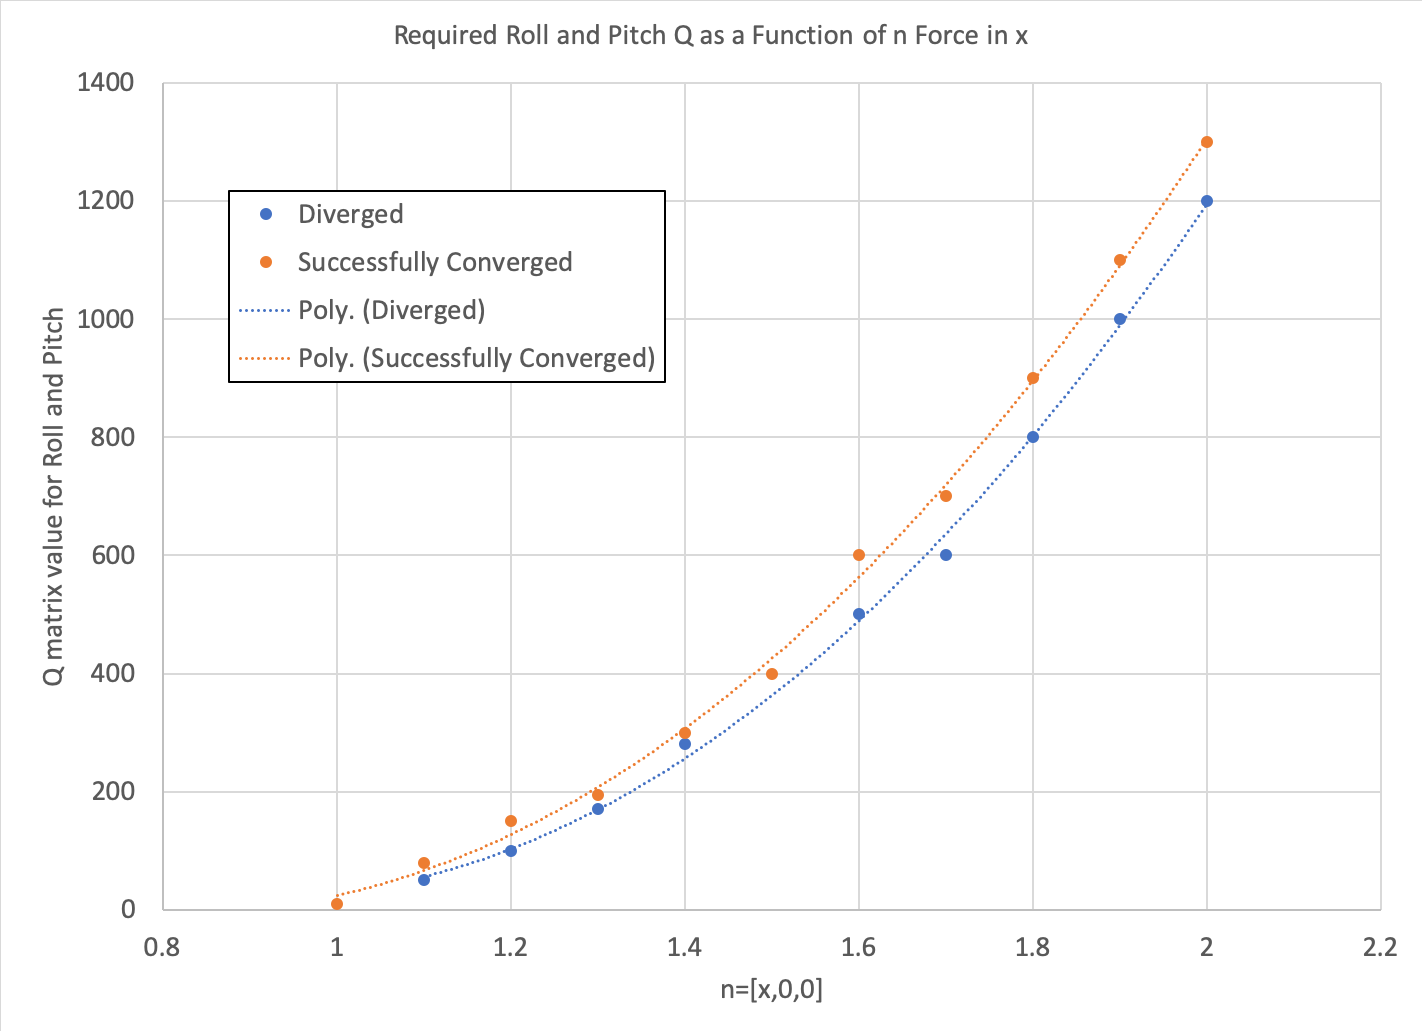
\includegraphics[width = 1\columnwidth]{images/RollPitch.png}
     \label{fig:Horizon}
     \caption{Q as Function of n in x}
\end{figure}
Figure \ref{Horizon} displays the results as well as approximates a control horizon (between the two lines) below which the system will not converge and above which it will.  Solutions close to the horizon exhibit often erratic flight prior to converging.  In the $n=(-n_1,0,0)$, the results were similar with convergence states in the opposite $x$ direction (as we would expect).  Forces, both positive and negative in the $n_2$ direction result in similar covergence states with the $x$ and $y$ positions transposed as seen in Table \ref{tab:STFCF1}.\\

\begin{table}[H] %[bp]
\begin{centering}
\begin{tabular}{|cccc|}
\hline
r & $Q_{(3,4/5)}$ & $z_{1-6}$   \\
\hline
 $[2,0,0]$&[1,1400]&[50.3,-0.2,1.5,0,-0.8,-0.6]\\
 $[-2,0,0]$&[1,1400]&[-50.0, 0.4. 3.3,0,1.0,0.1]\\
 $[0,2,0]$&[1,1400]&[-0.5, 50.0, 1.5,0.9,0,-0.2,]\\
 $[0,-2,0]$&[1,1400]&[0.6, -50.0,3.3,-0.9,0,-0.3]\\ 
\hline
\end{tabular}
\caption{State Variables from Constant Forces}
\label{tab:STFCF1}
\end{centering}
\end{table}

Convergences under forces in the $n_3$ direction benefit from strong $Q_{(4,4)}$ and $Q_{(5,5)}$ but can have far lower penalties before not converging.  Note in Table \ref{STFCF2} the closeness to the nest in $x$ and $y$ in the early scenarios (still $z$=2.8), while the state diverges at $Q_{(4,4)}=Q_{(5,5)}=145$.
\begin{table}[H] %[bp]
\begin{centering}
\begin{tabular}{|cccc|}
\hline
r & $Q_{(3,4/5)}$ & $z_{1-6}$   \\
\hline
 $[0,0,2]$&[1,1400]&[0.0, 0.0, 2.8,0,0,0]\\
 $[0,0,2]$&[1,1000]&[0.0, 0.0, 2.8,0,0,0]\\
$[0,0,2]$&[1,150]&[0.0, 0.0, 2.8,0,0,0.1]\\
$[0,0,2]$&[1,147]&[0.02, 0.01, 2.9,0,0,0.1]\\
$[0,0,2]$&[1,145]&[1.8, 0.5, 11.9, 0.2,-0.1,0.06]\\
 \hline
\end{tabular}
\caption{State Variables from Constant Forces}
\label{tab:STFCF2}
\end{centering}
\end{table}

\textbf{Moments}.  Similar to the above, we examined constant moments in each of the 3 directions.  At $n_1=.5$ (half mission parameter) we found near-convergence in the neighborhood of $Q_{(4,4)/(5,5)}=950$ with slight upward drift ($v_z>0$).  At $n_1=.5$ we could achieve convergence of the equations with $Q_{(4,4)/(5,5)}=1200$, but again not at the desire state.  Beyond, $n_1=.51$ it was increasingly not possible to converge on any state.  With $n_2$, the convergence horizon at $Q_{(4,4)}=Q_{(5,5)}=1200$ is between $.4875<n_2<.4885$.  Surprising to the team, the most sensitive was variation in $n_3$ where the convergence horizon for $Q_{(4,4)}=Q_{(5,5)}=Q_{(6,6)}=1000$ is between $.0445<n_3<.045$, an order of magnitude smaller. Thus it is impossible to meet mission parameters with both  $||n||<=1$ and $||r||<=2$, though it may be possible with only $r<2$.  Attempting this with a random, time dependent force at $Q_{(4,4)/(5,5)}=1400$, results in no convergence.  Though it gets close at times, the continued forces prevent velocity from converging enough for "shut down" as seen in Figure \ref{Randr}.
\begin{figure}[H]
\centering
\begin{subfigure}[b]{0.49\columnwidth}
    \centering
    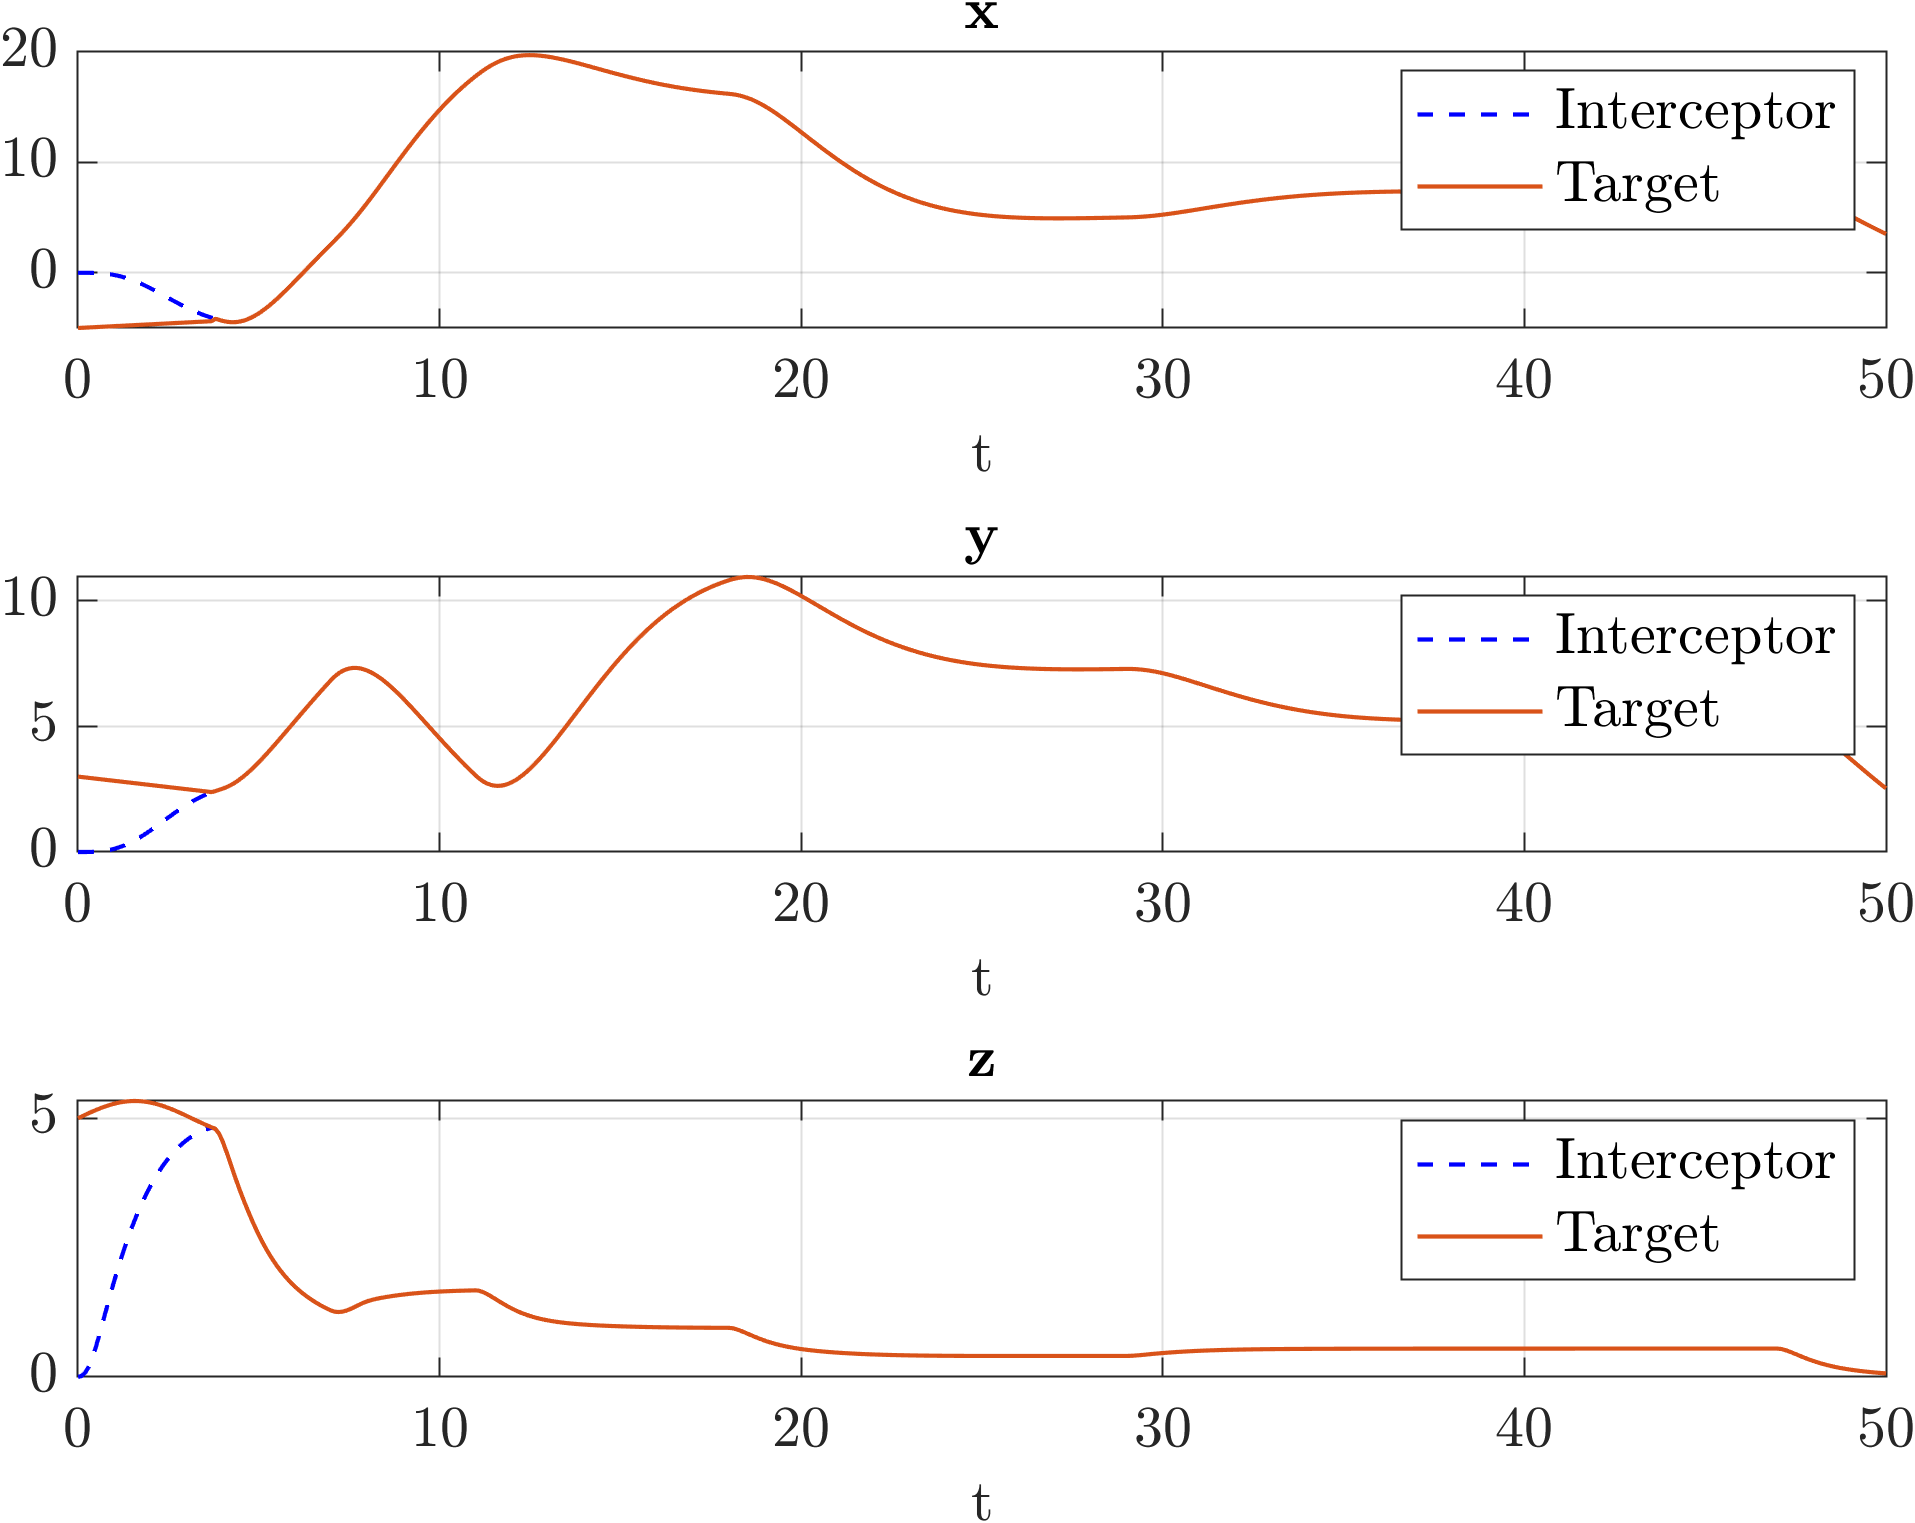
\includegraphics[width = 1\textwidth]{images/PosnRandom.png}
     \label{fig:PosRand}
     \vspace{-5mm}
     \caption{Positions}
\end{subfigure}
\begin{subfigure}[b]{0.49\columnwidth}
    \centering
    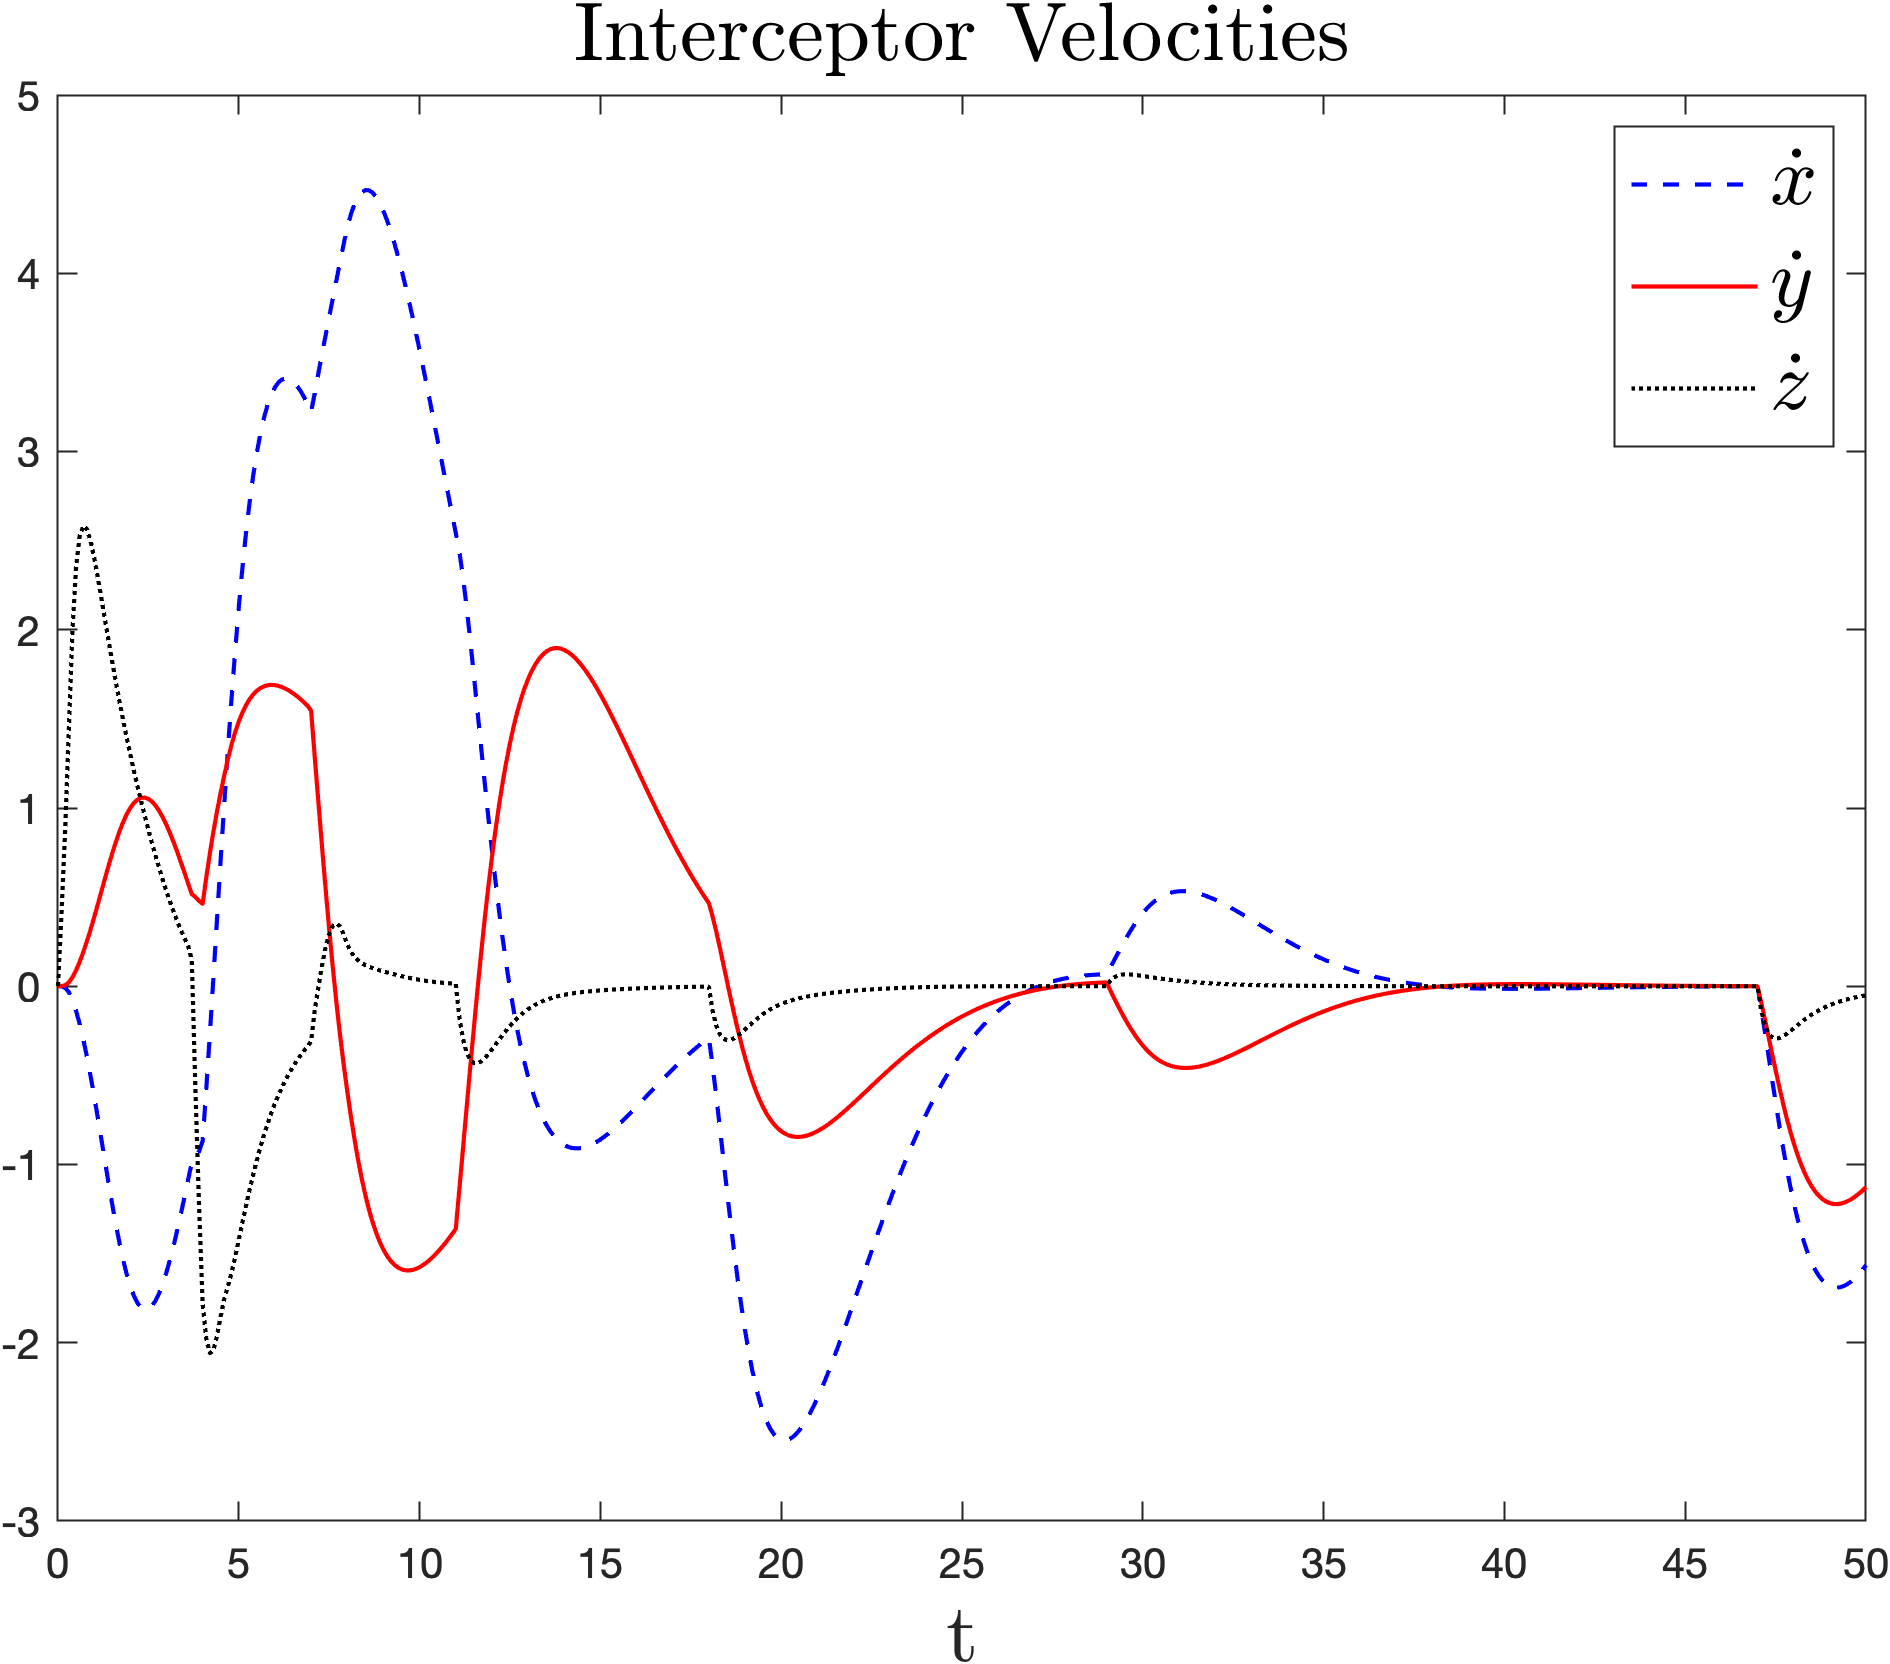
\includegraphics[width = 1\textwidth]{images/VelocityRandom.png}
     \label{fig:VRandom}
     \vspace{-5mm}
      \caption{Velocities}
 \end{subfigure}\\
 \bigskip
\begin{subfigure}[b]{1.0\columnwidth}
    \centering
    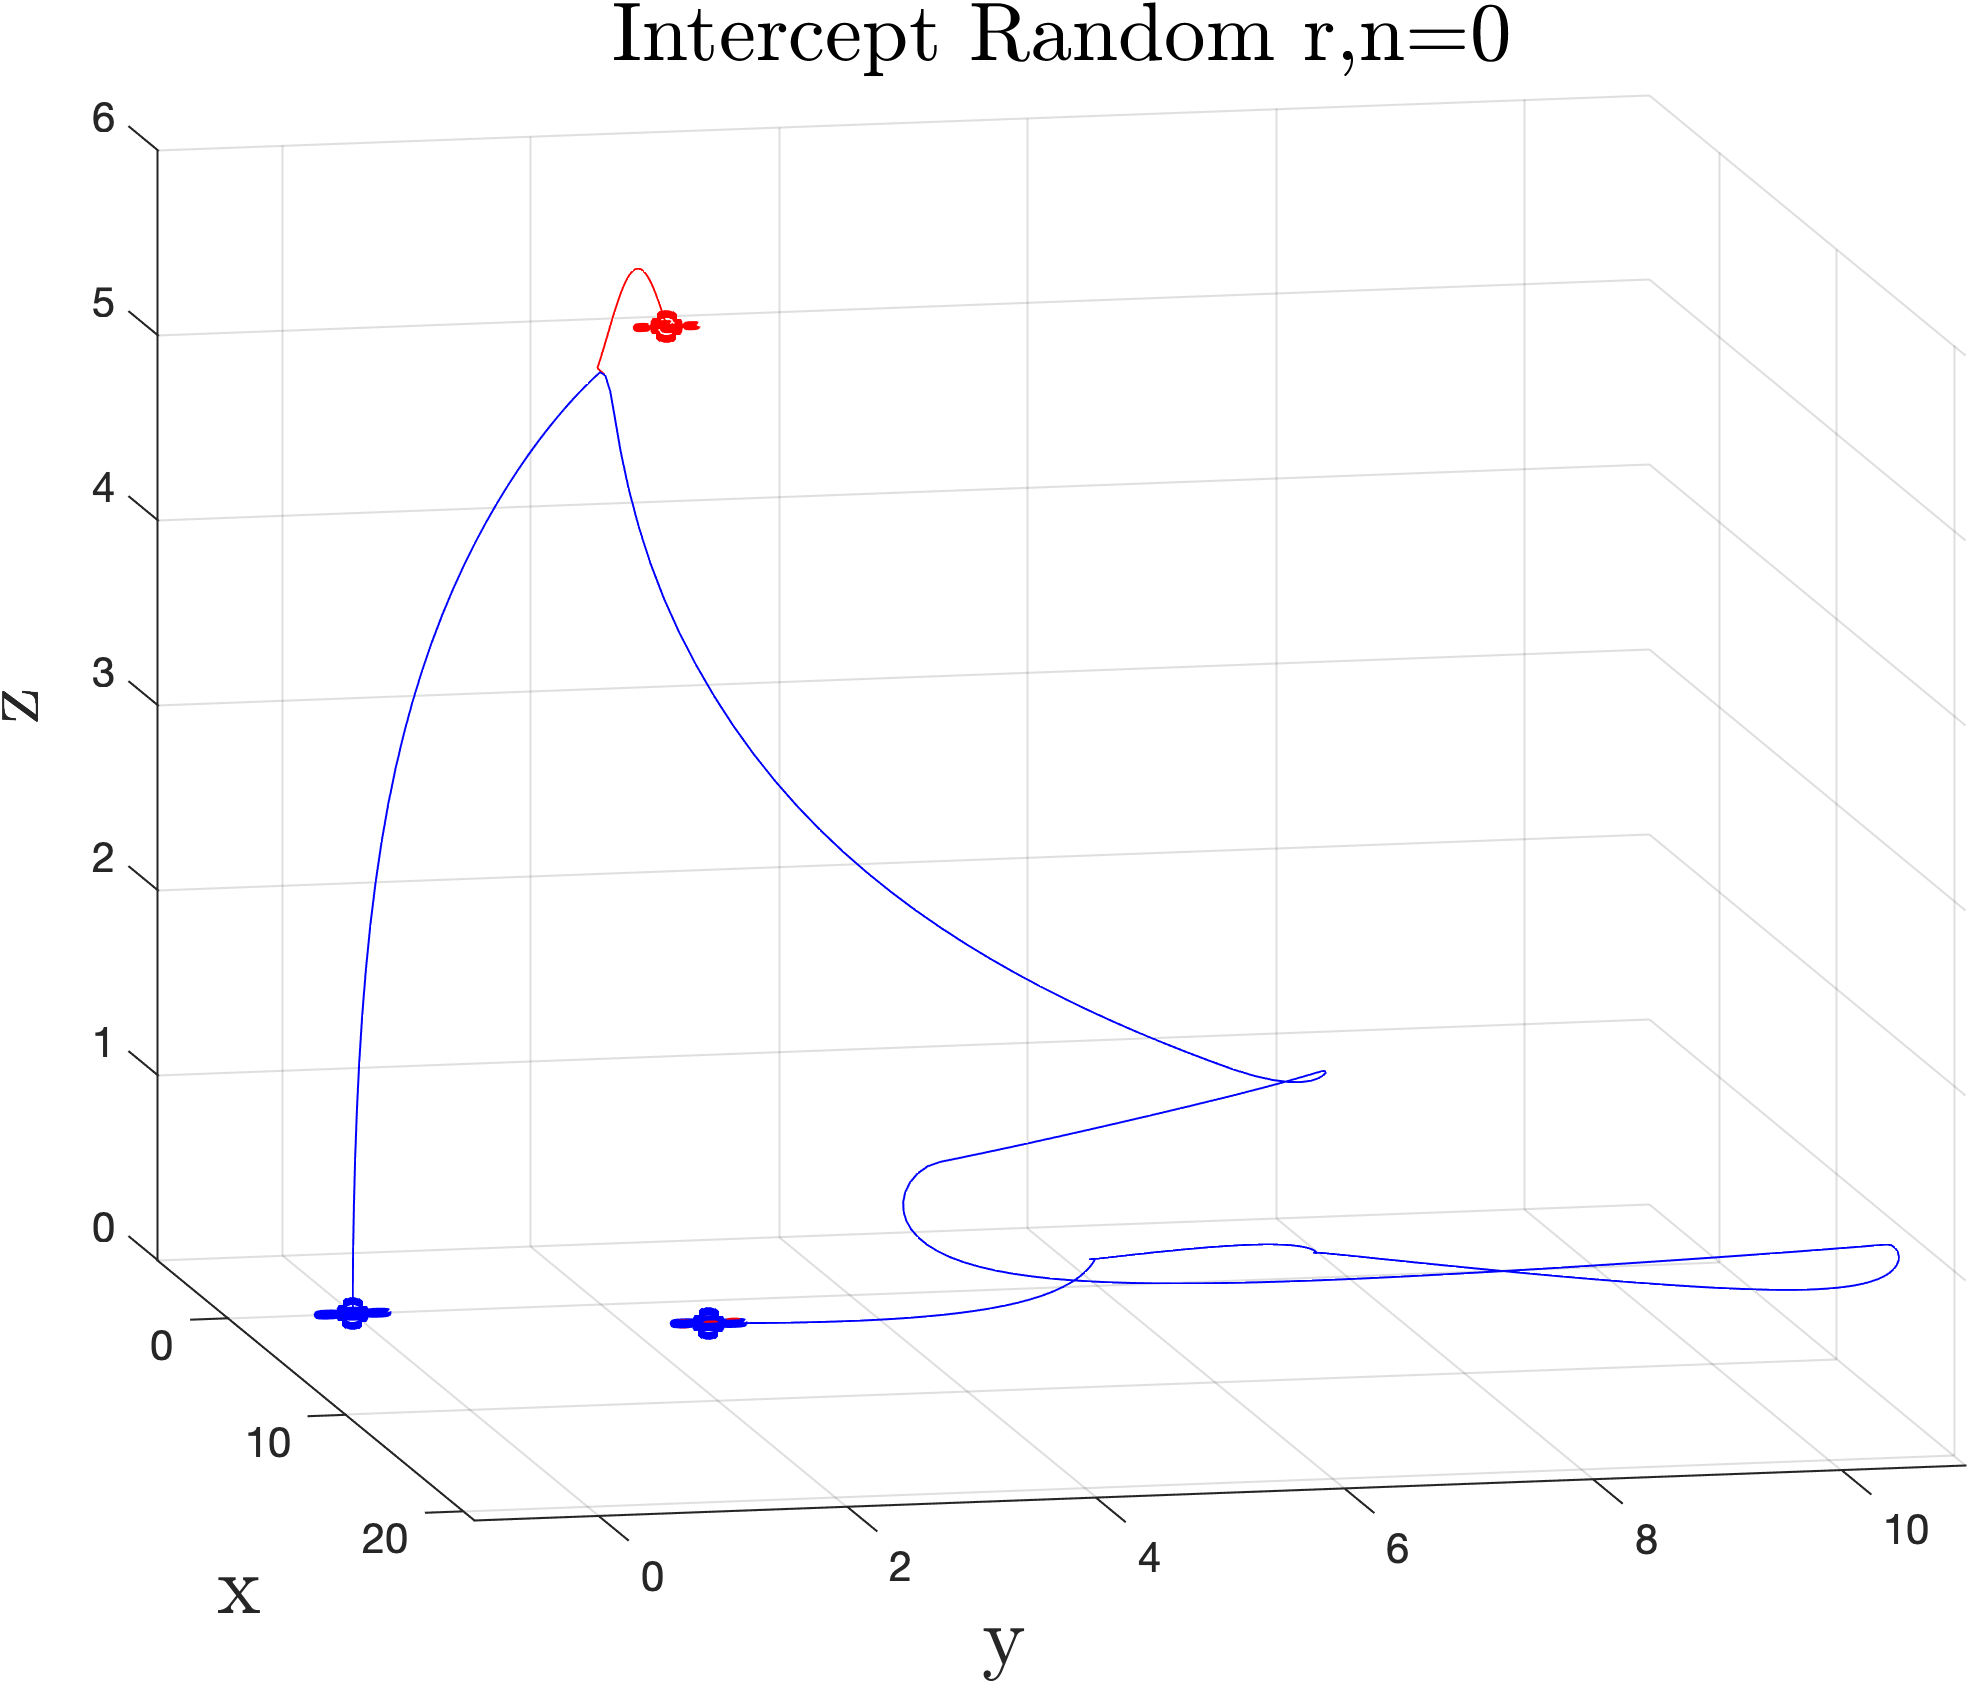
\includegraphics[width = 1\textwidth]{images/InterceptRandom.png}
     \label{fig:RandTraj}
     \vspace{-5mm}
     \caption{Trajectory}
 \end{subfigure}
    \caption{Random r Performance Tests}
     \label{fig:Randr}
\end{figure}
\section*{Discussion}
Further research would tune the Q and R matrices more closely.  Various external research suggests simply trial and error while others suggest optimization methods. A common method is to weight by the inverse of the maximum allowable error squared \cite{mur}.  We could also enhance the process to store target position to estimate the target velocity vector to anticipate next target position.  This could improve time to intercept and allow use of Q weightings for velocity components. More advanced analysis could include power analysis to improve battery life of the quadrotor to extend mission life.  
\label{References}
\bibliographystyle{abbrv}
\begin{thebibliography}{10}
\bibitem{JKim}
Jinho Kim, S. Andrew Gadsden, Stephen A . Wilkerson.
"A Comprehensive Survey of Control Strategies for Autonomus Quadrotors".
arXiv:2005.09858v1.
20 May 2020.
\bibitem{FaalP}
Faal, Siamak. Project Statement.  Class notes for RBE 502. Spring 2021.
\bibitem{FaalD}
Faal, Siamak. Notes on Control of Quadrotors. Class notes for RBE 502. March 3, 2021.
\bibitem{AHM}
Faraz Ahmad, Pushpendra Kumar, Anamika Bhandari, Pravin P. Patil.
Simulation of the Quadrotor Dynamics with LQR based Control.
Materials Today: Proceedings,Volume 24, Part 2, 2020, Pages 326-332,
ISSN 2214-7853.
https://doi.org/10.1016/j.matpr.2020.04.282.
\bibitem{OKY}
Okyere, E., Bousbaine, A., Poyi, G. T., Joseph, A. K., and Andrade.,
J. M. (2018) ‘LQR controller design for quad-rotor helicopters’,
The 9th International Conference on Power Electronics, Machines
and Drives. The Arena and Convention Centre, Liverpool, 17-19
April. London: The Institute of Engineering and Technology, pp.1-7
\bibitem{mur}
Murray, Richard M. Optimization Based Control.  California Institute of Technology. January 4th, 2010.




\end{thebibliography}

\end{multicols}

\end{document}
